%%%%%%%%%%%%%%%%%%%%%%%%%%%%%%%%%%%%%%%%%%%%%%%%%%%%%%%%%%%%%%%%%%%%%%%%%%
%%LaTeX template for papers && theses									%%
%%Done by the incredible ||Z01db3rg||									%%
%%Under the do what ever you want license								%%
%%%%%%%%%%%%%%%%%%%%%%%%%%%%%%%%%%%%%%%%%%%%%%%%%%%%%%%%%%%%%%%%%%%%%%%%%% 

%start preamble
\documentclass[paper=a4,fontsize=11pt]{scrartcl}%kind of doc, font size, paper size
\usepackage[ngerman]{babel}%for special german letters etc			
%\usepackage{t1enc} obsolete, but some day we go back in time and could use this again
\usepackage[T1]{fontenc}%same as t1enc but better						
\usepackage[utf8]{inputenc}%utf-8 encoding, other systems could use others encoding
%\usepackage[latin9]{inputenc}			
\usepackage{amsmath}%get math done
\usepackage{amsthm}%get theorems and proofs done
\usepackage{graphicx}%get pictures & graphics done
\graphicspath{{pictures/}}%folder to stash all kind of pictures etc
\usepackage[pdftex,hidelinks]{hyperref}%for links to web
\usepackage{amssymb}%symbolics for math
\usepackage{amsfonts}%extra fonts
\usepackage []{natbib}%citation style
\usepackage{caption}%captions under everything
\usepackage{listings}
\usepackage[titletoc]{appendix}
\numberwithin{equation}{section} 
\usepackage[printonlyused,withpage]{acronym}%how to handle acronyms
\usepackage{float}%for garphics and how to let them floating around in the doc
\usepackage{cclicenses}%license!
\usepackage{xcolor}%nicer colors, here used for links
\usepackage{wrapfig}%making graphics floated by text and not done by minipage
\usepackage{dsfont}
\usepackage{stmaryrd}
\usepackage{geometry}
\usepackage{hyperref}
\usepackage{fancyhdr}
\usepackage{menukeys}
\usepackage{multicol}

\pagestyle{fancy}
\lhead{Benjamin Tröster\\Netzwerke Übung (WiSe2018/19)}
\rhead{FB 4 -- Angewandte Informatik\\ HTW-Berlin}
\lfoot{Übungsblatt 2 -- Netzwerke Grundlagen}
\cfoot{}
\fancyfoot[R]{\thepage}
\renewcommand{\headrulewidth}{0.4pt}
\renewcommand{\footrulewidth}{0.4pt}

\lstdefinestyle{Bash}{
  language=bash,
  showstringspaces=false,
  basicstyle=\small\sffamily,
  numbers=left,
  numberstyle=\tiny,
  numbersep=5pt,
  frame=trlb,
  backgroundcolor=\color{gray!20},
  %linewidth=0.9\linewidth,
  %xleftmargin=0.5\linewidth
  %upquote=true,
  columns=fullflexible,
  literate={*}{{\char42}}1
         {-}{{\char45}}1
}


\newlength\labelwd
\settowidth\labelwd{\bfseries viii.)}
\usepackage{tasks}
\settasks{counter-format =tsk[a].), label-format=\bfseries, label-offset=3em, label-align=right, label-width
=\labelwd, before-skip =\smallskipamount, after-item-skip=0pt}
\usepackage[inline]{enumitem}
\setlist[enumerate]{% (
labelindent = 0pt, leftmargin=*, itemsep=12pt, label={\textbf{\arabic*.)}}}

\pdfpkresolution=2400%higher resolution

%settings colors for links
%\hypersetup{
 %   colorlinks,
  %  linkcolor={blue!50!black},
   % citecolor={blue},
    %urlcolor={blue!80!black}
%}

%\usepackage[pagetracker=true]{biblatex}

%%here begins the actual document%%
\newcommand{\horrule}[1]{\rule{\linewidth}{#1}} % Create horizontal rule command with 1 argument of height


\DeclareMathOperator{\id}{id}

\title{	
\normalfont \normalsize 
\textsc{Übungsblatt 2}
}

\begin{document}
\begin{center}
\Large{\textbf{Übungsblatt 02 -- Netzwerkgrundlagen}}
\end{center}
Sie lernen die Raspberry Pis kennen, bauen ein eigenes Netzwerk physisch auf, nehmen die IP-Konfiguration des Netzes via Kommandozeile um.
\begin{center}\Large{\textbf{Aufgabe A - Raspberry Pi}}\end{center}\vskip0.25in
\textbf{Kommandos:}
\begin{multicols}{3}
\begin{itemize}
	\item ifconfig/ip addr
	\item systemctl
	\item sudo
\end{itemize}
\end{multicols}
\begin{itemize}
	\item[0.)] Bauen Sie Ihren Raspberry Pi zusammen. Vergewissern Sie sich, dass alle Komponenten korrekt zusammengesetzt wurden!
	\item[1.)] Schalten Sie Ihre Raspberry Pis an! Sie werden automatisch eingeloggt.
	\item[2.)] Finden sich kurz auf der Commandline zurecht: \glqq Wer bin ich, wo bin ich, auf welchem Gerät bin ich?\grqq
		\begin{lstlisting}[style=Bash, language=Bash]
whoami
pwd
hostname
		\end{lstlisting}	
	\item[3.)] Lassen Sie sich den Status des DHCP und Networking-Service anzeigen.
	\begin{lstlisting}[style=Bash, language=Bash]
sudo systemctl status dhcpcd
		\end{lstlisting}
	\item[4.)] Falls der DHCP-Service ausgeschaltet sein sollte, können Sie diesen mit dem Script \emph{nw\_default.sh} wie folgt einschalten:
	\begin{lstlisting}[style=Bash, language=Bash]
./nw_default.sh
		\end{lstlisting}	
	\item[5.)] \textbf{Wenn Sie ihre eigene $\mu$-SD-Karte (Micro-SD) nutzen, können Sie das Standardpasswort ändern (Wie das funktioniert steht in der Man-Page: passwd).}
		\begin{lstlisting}[style=Bash, language=Bash]
# abfrage des alten password und setzen des neuen
passwd
# aendern des password fuer user vivek
passwd vivek
		\end{lstlisting}	
	\item[6.)] Lassen Sie sich mit den Kommandos:
\begin{lstlisting}[style=Bash, language=Bash]
uname -or
#bsp Ausgabe:
4.15.14-1-ultra_kernel GNU/Linux # Linux Kernel 4.13.14-1 mit modifizierten Kernel
\end{lstlisting} und
		
\begin{lstlisting}[style=Bash, language=Bash]
cat /etc/os-release
#Bsp. Ausgabe:
NAME="Arch Linux"
PRETTY_NAME="Arch Linux"
ID=arch
ID_LIKE=archlinux
ANSI_COLOR="0;36"
HOME_URL="https://www.archlinux.org/"
SUPPORT_URL="https://bbs.archlinux.org/"
BUG_REPORT_URL="https://bugs.archlinux.org/"
\end{lstlisting} anzeigen, welcher Betriebssystemkern (Kernel) und welche Distribution auf dem Raspberry Pi läuft.
	\item[7.)] Nutzen Sie diese Information um im Falle von Fehlern/ Fehlkonfigurationen für das Betriebssystem zu recherchieren, wie Sie Tools nutzen und Einstellungen vornehmen. Es ist schlau in einer Suche den Namen des Betriebssystems vorkommen zu lassen. Sie wollen keine Windowslösungen finden.
	\item[8.)] In der letzten Laborübung haben Sie bereits begonnen sich ein Cheat-Sheet zu schreiben. Dieses können Sie weiterentwickeln. Mit folgendem Befehl kopieren Sie den Ordner der letzten Übung. 
	\begin{lstlisting}[style=Bash, language=Bash]
scp -r s0xxxxxx@uranus.f4.htw-berlin.de:~/exercise_notes/tutorials/ ~/
		\end{lstlisting}
		Darüber hinaus sind einige Cheat-Sheets im Ordner \path{~/todo} verfügbar.
\end{itemize}
\vskip0.5in

\begin{center}
\Large{\textbf{Aufgabe B - Anzeige der bestehenden Netzwerkkonfiguration}}
\end{center}\vskip0.25in
Bevor Sie ein eigenes kleines Netzwerk einrichten, sollen Sie sich vertrauter mit den dafür Notwendigen Tools machen. Daher soll zunächst die bestehende Netzwerkkonfiguration untersucht werden.\\
\textbf{Kommandos}
\begin{multicols}{3}
\begin{itemize}
	\item ifconfig/ip addr
	\item ip link
	\item systemctl
	\item ping
\end{itemize}
\end{multicols}
Eine aktive Netzwerkverbindung ist Voraussetzung für die Kommunikation zwischen Rechnern in einem Netzwerk. Jeder Rechner muss hierfür eine passende IP-Adresse haben, mit der er andere Rechner im Netz erreichen kann. 
\begin{itemize}
	\item[1.)] Lassen Sie sich die aktuelle IP-Adresskonfiguration anzeigen.
	\begin{lstlisting}[style=Bash, language=Bash]
ip addr 	#zeigt alle geraete
ip addr show eth0 # zeigt nur konfig. von eth0
ifconfig # zeigt alle geraete
ifconfig eth0 # zeigt konfig. von eth0
		\end{lstlisting}
		
		\begin{lstlisting}[style=Bash, language=Bash]
#Bsp fuer Loopback und ethernet mit ipv4 & ipv6:
ip addr 	
1: lo: <LOOPBACK,UP,LOWER_UP> mtu 65536 qdisc noqueue state UNKNOWN 
							group default qlen 1000
    link/loopback 00:00:00:00:00:00 brd 00:00:00:00:00:00
    inet 127.0.0.1/8 scope host lo
       valid_lft forever preferred_lft forever
    inet6 ::1/128 scope host 
       valid_lft forever preferred_lft forever
2: eth0: <BROADCAST,MULTICAST,UP,LOWER_UP> mtu 1500 qdisc fq_codel
							state UP group default qlen 1000
    link/ether ac:22:0b:4f:45:8c brd ff:ff:ff:ff:ff:ff
    inet 192.168.178.22/24 brd 192.168.178.255 scope global
    							dynamic noprefixroute eno1
       valid_lft 857067sec preferred_lft 857067sec
    inet6 ****:8109:****:****:****:****:****:e863/64 scope global
    							dynamic noprefixroute 
       valid_lft 5303sec preferred_lft 2603sec
    inet6 fe80::3911:17c4:34a6:fd1d/64 scope link noprefixroute 
       valid_lft forever preferred_lft forever
		\end{lstlisting}
	\item[2.)] Wo finden Sie in der Ausgabe die folgenden Informationen:
	\begin{tasks}(1)
		\task~ MAC-Adresse der Netzwerkkarte
		\task~ Aktuelle IP-Adresse des Systems
		\task~ Subnetzmaske
		\task~ Besteht eine aktive Verbindung mit dem Netzwerk (also Kabel mit dem Switch verbunden)?
		\task~ Qualität der Verbindung? (Anzahl fehlerhafter Pakete)
		\task~ Übertragene Datenmenge?
	\end{tasks}
	\begin{lstlisting}[style=Bash, language=Bash]
#zu a)
# einfach und ausreichend
ip -o link
# fuer fortgeschrittene
cat /sys/class/net/*/address # zeigt alle MAC Adressen an
# etwas komplizierter, mit regex:
ifconfig eth0 | grep -o -E '([[:xdigit:]]{1,2}:){5}[[:xdigit:]]{1,2}'
ip link show eth0 | awk '/ether/ {print $2}'
	\end{lstlisting}
		
\begin{lstlisting}[style=Bash, language=Bash]
#zu b)
# einfache Loesung schauen Sie nach dem Wort inet bzw. inet6 fuer ipv6
ip addr show eth0 
# bzw
ifconfig eth0
# fuer fortgeschrittene
ip addr show eth0 | awk '/inet/ {print $2}'# IPv4 & 6
ip addr show eth0 | awk '/inet6/ {print $2}'#nur IPv4
ifconfig eth0 | awk '/netmask/ {print $2}'
	\end{lstlisting}	
		
	\begin{lstlisting}[style=Bash, language=Bash]
#zu c)
# schauen Sie ebenfalls beim Eintrag von inet 
ip addr show eth0 # in CIDR notation
# bzw direkt unter dem Eintrag netmask:
ifconfig eth0
# fuer fortgeschrittene
ip addr show eht0 | awk '/inet/ {print $2}' # CIDR notation
ifconfig eth0 | awk '/netmask/ {print $4}'
	\end{lstlisting}
		
	\begin{lstlisting}[style=Bash, language=Bash]
#zu d)
# Im Zweifelsfall direkt an den Geraeten - LEDs
# oder: 
netstat -natp
netstat -tulpn
netstat -s
ss -s
	\end{lstlisting}
		
\begin{lstlisting}[style=Bash, language=Bash]
#zu e)
#einfache Loesung - direkt unter dem Eintrag error & dropped:
ifconfig eth0 
#fuer fortgeschrittene
ifconfig eth0 | awk '/errors/ {print $3}'
ifconfig eth0 | awk '/dropped/ {print $3}'
ifconfig | grep -E "^\w|errors.* " | sed 's/pack.*errors:/Errors:/g'
| sed 's/ drop.*//g' | sed 's/HW.*//g'
#Achtung Ein-Zeiler die Single-Quotes muessen angepasst werden
	\end{lstlisting}	
		
	\begin{lstlisting}[style=Bash, language=Bash]
#zu f)
#einfache Loesung - direkt unter dem Eintrag packets & bytes:
ifconfig eth0 
#fuer fortgeschrittene
ifconfig eth0 | awk '/bytes/ {print $0}'
nload
cat /proc/net/dev
netstat -i
cat /sys/class/net/eth0/statistics/rx_bytes
	\end{lstlisting}	
	\item[3.)] Prüfung ob ein Netzwerkverbindung besteht. Zum Prüfen können Sie folgende Aktionen durchführen:
	\begin{tasks}
		\task~ Webbrowser öffnen und versuchen eine Seite anzuzeigen (dazu muss der Rechner eine IP-Adresse
haben, sein Gateway kennen und das DNS richtig konfiguriert sein, der Webserver muss aktiv sein, keine Firewall darf die Pakete blocken).
		\task~ Auf der Kommandozeile einen Rechner mit seinen Namen anpingen (bspw.: \url{htw-berlin.de}).
		\task~ Ping auf eine IP-Adresse.
		\task~ Ping auf die IP-Adresse des Routers (IP: 10.10.10.254) -- funktioniert die Kommunikation im lokalen Netz (LAN)?
		\task~ Ping auf die eigene IP-Adresse -- wurde der lokale Netzwerkstack richtig gestartet?
	\end{tasks}
	\begin{lstlisting}[style=Bash, language=Bash]
#zu b)
# Sende 3 Pakete nacheinander an Adresse
ping -c3 www.htw-berlin.de
# sehr schoener hostname!
PING moehre.htw-berlin.de (141.45.7.250) 56(84) bytes of data.
64 bytes from moehre.htw-berlin.de (141.45.7.250): icmp_seq=1 ttl=245 time=15.4 ms
64 bytes from moehre.htw-berlin.de (141.45.7.250): icmp_seq=2 ttl=245 time=11.8 ms
64 bytes from moehre.htw-berlin.de (141.45.7.250): icmp_seq=3 ttl=245 time=11.1 ms

--- moehre.htw-berlin.de ping statistics ---
3 packets transmitted, 3 received, 0% packet loss, time 2002ms
rtt min/avg/max/mdev = 11.159/12.830/15.440/1.871 ms
	\end{lstlisting}
		
	\begin{lstlisting}[style=Bash, language=Bash]
#zu c)
ping -c3 8.8.8.8 # google dns oder 
ping -c3 141.45.146.48 # uranus server der htw
# Laesst kein ping/ICMP zu
ping -c3 -p 22 uranus.f4.htw-berlin.de
PATTERN: 0x22
PING uranus.f4.htw-berlin.de (141.45.146.48) 56(84) bytes of data.

--- uranus.f4.htw-berlin.de ping statistics ---
3 packets transmitted, 0 received, 100% packet loss, time 2077ms

	\end{lstlisting}
	\begin{lstlisting}[style=Bash, language=Bash]
#zu d)
ping -c3 10.10.10.254
	\end{lstlisting}
		
	\begin{lstlisting}[style=Bash, language=Bash]
#zu e)
ping -c3 127.0.0.1 # bzw.
ping -c3 localhost
PING localhost(localhost (::1)) 56 data bytes
64 bytes from localhost (::1): icmp_seq=1 ttl=64 time=0.026 ms
64 bytes from localhost (::1): icmp_seq=2 ttl=64 time=0.027 ms
64 bytes from localhost (::1): icmp_seq=3 ttl=64 time=0.026 ms

--- localhost ping statistics ---
3 packets transmitted, 3 received, 0% packet loss, time 2026ms
rtt min/avg/max/mdev = 0.026/0.026/0.027/0.004 ms

	\end{lstlisting}	
	\item[4.)] Schalten Sie den DHCP-Dienst permanent aus.
	\begin{lstlisting}[style=Bash, language=Bash]
sudo systemctl status dhcpcd
sudo systemctl stop dhcpcd
sudo systemctl disable dhcpcd
		\end{lstlisting}	
	\item[5.)] Schalten Sie den Networking-Service permanent ein und starten Sie den Raspberry Pi neu.
	\begin{lstlisting}[style=Bash, language=Bash]
sudo systemctl enable networking.service
reboot
	\end{lstlisting}	
\end{itemize}

\begin{center}\Large{\textbf{Aufgabe C - Switched LAN}}\end{center}\vskip0.25in
In der Hausaufgabe haben Sie ein kleines Netzwerk geplant, dies soll in Vierergruppen mit der vorhandenen Hardware umgesetzt werden.
\begin{itemize}
	\item[1.)] Beschriften Sie die Skizze aus der Planungsphase mit Gerätename und evtl. den Namen der Gruppenmitglieder.
	\begin{figure}[H]
	\centering
	\includegraphics[scale=0.5]{switched_nw}
	\end{figure}
	\item[2.)]  Wählen Sie eine Netzwerkadresse/ IP-Adresse (IP address) und Subnetzmaske. Das Netzwerk sollte der IP-Range 10.0.X.Y genügen. D.h. $X$ ist durch ihre Bankreihe bestimmt und $Y$ entspricht dem Host. Die IP-Adressen 10.0.0.0, 10.0.0.254 und 10.0.0.255 können nicht belegt werden.
	\begin{table}[H]
\centering
\caption{Beispielkonfiguration}
\label{my-label}
\begin{tabular}{cccc}
\textbf{Gruppe} & \textbf{Netzwerk IP} & \textbf{Subnetzmaske} & \textbf{CIDR}\\ 
Fractals & 10.1.1.0 & 255.255.255.248 & 10.1.1.0/29  \\
1337 & 10.1.2.0 & 255.255.255.248 & 10.1.2.0/29 \\
... & & &
\end{tabular}
\end{table}
	\item[3.)] Vergeben Sie für jeden Raspberry Pi eine IP-Adresse und tragen diese auf der Skizze ein.
	\begin{figure}[H]
	\centering
	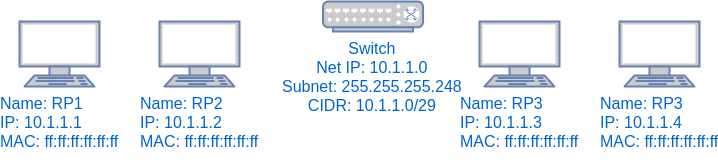
\includegraphics[scale=0.5]{switched_nw_full}
\end{figure}		
	\item[2.)] Bringen Sie die MAC-Adresse Ihres Raspberry Pis in Erfahrung und notieren Sie diese auf der Skizze.
	\begin{lstlisting}[style=Bash, language=Bash]
#s.o.
ifconfig eth0
# oder in schoen
ip addr show eht0 | awk '/inet/ {print $2}' # CIDR notation
ifconfig eth0 | awk '/netmask/ {print $4}'
#bsp Ausgabe:
255.255.255.0
	\end{lstlisting}
	\item[3.)] Umsetzen der Konfiguration
\begin{tasks}[counter-format=(tsk[r])](1)
	\task~ Lassen Sie sich im Terminal die aktuelle Netzwerkkonfiguration mit \emph{ifconfig} und \emph{ip addr} anzeigen. Haben Sie schon eine IP-Adresse (inet) und Subnetzmaske (netmask)?
	\task~ Richten Sie die Raspberry Pis mit den Befehlen den Ihnen bekannten Befehle ein und notieren Sie sich die Kommandos in Ihrem Cheat-Sheet.
	\task~ Lassen Sie sich im Terminal die neue Netzwerkkonfiguration mit \emph{ifconfig} oder \emph{ip addr} anzeigen.
\end{tasks}
\begin{lstlisting}[style=Bash, language=Bash]
#zu i)
# IP & subnet mask sollte nach reboot nicht vergeben sein
ip addr show eth0
ifconfig eth0
	\end{lstlisting}
		\begin{lstlisting}[style=Bash, language=Bash]
#zu ii)
# via iproute2
ip addr add 10.1.1.1/29 dev eth0
ip link set eth0 up
# via net tools
ifconfig eth0 10.1.1.1 netmask 255.255.255.248 up
	\end{lstlisting}
	\begin{lstlisting}[style=Bash, language=Bash]
#zu iii)
# IP & subnet mask sollte nun vergeben sein
ip addr show eth0
ifconfig eth0
	\end{lstlisting}
\item[4.)] Testen des Netzes
\begin{tasks}[counter-format=(tsk[r])](1)
	\task~ Testen Sie, ob Sie ihre Raspberry Pis gegenseitig mit dem Befehl \emph{ping} \glqq anpingen\grqq\ können. Lassen Sie dabei einen der drei Anderen Raspberry Pis außen vor und merken Sie sich welcher das war.
	\task~ Starten Sie Ihren Raspberry Pi per Kommandozeile neu. Pingen Sie einen der beiden bereits \glqq angepingten\grqq\ Raspberry Pis erneut an. Funktioniert es immer noch?\\
	Dies sollte nicht mehr funktionieren, da Ihre Konfiguration nur \glqq on the fly\grqq\ vorgenommen worden ist und nach einem Neustart dem System nicht mehr bekannt ist.
	\task~ Lassen Sie sich die Netzwerkkonfiguration anzeigen.\\
	s.o.
	\task~ Setzen Sie eine persistente Netzwerkkonfiguration mittels Dateien um. Nutzen Sie dabei einen Commandline-Editor ihrer Wahl z.B. \emph{vim} oder \emph{emacs}.
\end{tasks}
\begin{lstlisting}[style=Bash, language=Bash]
#zu iv)
# /etc/network/interfaces
auto lo # automatische setzen des loopback devices (localhost)
iface lo inet loopback # setze loopback ipv4 adresse

auto eth0 # hochfahren des interfaces zur boot zeit
allow-hotplug eth0 # erlaubt kabel wechsel waehrend des betriebs
iface eth0  inet static # statische ip addr fuer interface eth0
	address 10.1.1.1 # ip addr - statisch
	netmask 255.255.255.248 # subnetzmaske
	\end{lstlisting}
\end{itemize}
\end{document}